\begin{figure}[!htb]
\begin{center}
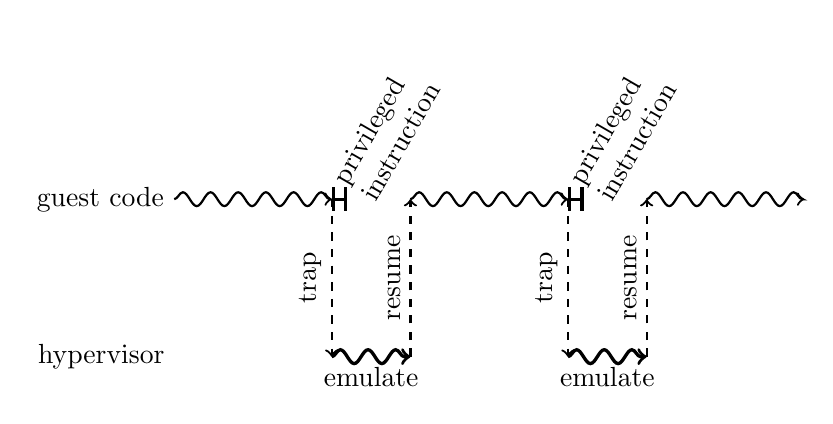
\begin{tikzpicture}


\draw[thick, decorate, decoration=snake, ->] (0, 2) -- (2, 2) node at (0,2) [left] {guest code};
\draw[very thick, |-|] (2, 2) -- (2.2, 2) node [above, right, rotate=60, text width=2cm]{privileged instruction};

\node at (0,0) [left] {hypervisor};
\draw[thick, dashed, ->] (2, 2) -- (2, 0) node [above, align=center,midway, rotate=90]{trap};
\draw[very thick, decorate, decoration=snake, ->] (2.0, 0) -- (3, 0) node [below,midway] {emulate};
\draw[thick, dashed, ->] (3, 0) -- (3, 2) node [above, align=center, midway, rotate=90] {resume};

\draw[thick, decorate, decoration=snake, ->] (3, 2) -- (5, 2);
\draw[very thick, |-|] (5, 2) -- (5.2, 2) node [above, right, rotate=60, text width=2cm]{privileged instruction};

\draw[thick, dashed, ->] (5, 2) -- (5, 0) node [above, align=center,midway, rotate=90]{trap};
\draw[very thick, decorate, decoration=snake, ->] (5, 0) -- (6, 0)  node [below,midway] {emulate};
\draw[thick, dashed, ->] (6, 0) -- (6, 2) node [above, align=center,midway, rotate=90]{resume};

\draw[thick, decorate, decoration=snake, ->] (6, 2) -- (8, 2);

\end{tikzpicture}
\end{center}
\ifreport
\caption{Faithful Virtualization (trap-and-emualte)}
\fi
\label{fig-virt-faithful}
\end{figure}
